% Graphic for TeX using PGF
% Title: C:\Users\CAMUGLIAL_INFO\Desktop\Diplome\Diplome\_Documentation\Diagrammes\Connexion.dia
% Creator: Dia v0.97.2
% CreationDate: Fri May 26 08:34:40 2017
% For: admintech
% \usepackage{tikz}
% The following commands are not supported in PSTricks at present
% We define them conditionally, so when they are implemented,
% this pgf file will use them.
\ifx\du\undefined
  \newlength{\du}
\fi
\setlength{\du}{15\unitlength}
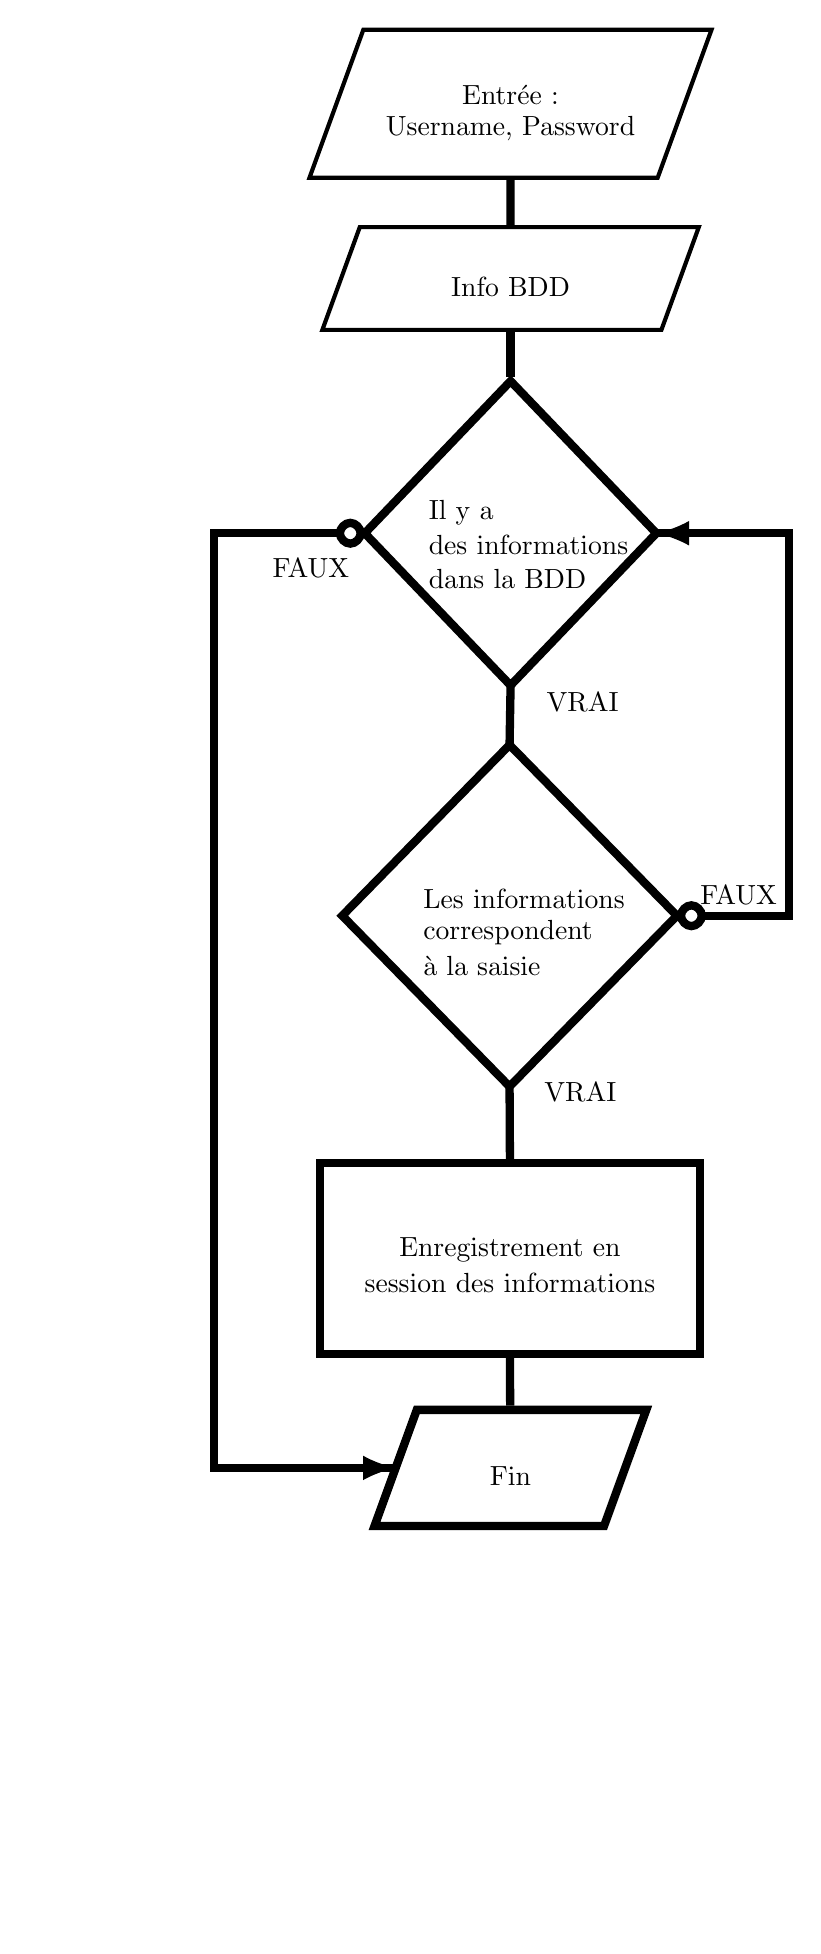
\begin{tikzpicture}
\pgftransformxscale{1.000000}
\pgftransformyscale{-1.000000}
\definecolor{dialinecolor}{rgb}{0.000000, 0.000000, 0.000000}
\pgfsetstrokecolor{dialinecolor}
\definecolor{dialinecolor}{rgb}{1.000000, 1.000000, 1.000000}
\pgfsetfillcolor{dialinecolor}
% setfont left to latex
\definecolor{dialinecolor}{rgb}{0.000000, 0.000000, 0.000000}
\pgfsetstrokecolor{dialinecolor}
\node[anchor=west] at (13.491129\du,10.889792\du){};
\definecolor{dialinecolor}{rgb}{1.000000, 1.000000, 1.000000}
\pgfsetfillcolor{dialinecolor}
\fill (21.590643\du,2.192741\du)--(29.977996\du,2.192741\du)--(28.680748\du,5.756900\du)--(20.293395\du,5.756900\du)--cycle;
\pgfsetlinewidth{0.100000\du}
\pgfsetdash{}{0pt}
\pgfsetdash{}{0pt}
\pgfsetmiterjoin
\definecolor{dialinecolor}{rgb}{0.000000, 0.000000, 0.000000}
\pgfsetstrokecolor{dialinecolor}
\draw (21.590643\du,2.192741\du)--(29.977996\du,2.192741\du)--(28.680748\du,5.756900\du)--(20.293395\du,5.756900\du)--cycle;
% setfont left to latex
\definecolor{dialinecolor}{rgb}{0.000000, 0.000000, 0.000000}
\pgfsetstrokecolor{dialinecolor}
\node at (25.135696\du,3.769820\du){Entrée : };
% setfont left to latex
\definecolor{dialinecolor}{rgb}{0.000000, 0.000000, 0.000000}
\pgfsetstrokecolor{dialinecolor}
\node at (25.135696\du,4.569820\du){Username, Password};
% setfont left to latex
\definecolor{dialinecolor}{rgb}{0.000000, 0.000000, 0.000000}
\pgfsetstrokecolor{dialinecolor}
\node[anchor=west] at (25.135696\du,3.974820\du){};
\definecolor{dialinecolor}{rgb}{1.000000, 1.000000, 1.000000}
\pgfsetfillcolor{dialinecolor}
\fill (21.504495\du,6.947608\du)--(29.671666\du,6.947608\du)--(28.770623\du,9.423204\du)--(20.603452\du,9.423204\du)--cycle;
\pgfsetlinewidth{0.100000\du}
\pgfsetdash{}{0pt}
\pgfsetdash{}{0pt}
\pgfsetmiterjoin
\definecolor{dialinecolor}{rgb}{0.000000, 0.000000, 0.000000}
\pgfsetstrokecolor{dialinecolor}
\draw (21.504495\du,6.947608\du)--(29.671666\du,6.947608\du)--(28.770623\du,9.423204\du)--(20.603452\du,9.423204\du)--cycle;
% setfont left to latex
\definecolor{dialinecolor}{rgb}{0.000000, 0.000000, 0.000000}
\pgfsetstrokecolor{dialinecolor}
\node at (25.137559\du,8.380406\du){Info BDD};
\definecolor{dialinecolor}{rgb}{1.000000, 1.000000, 1.000000}
\pgfsetfillcolor{dialinecolor}
\fill (25.137559\du,10.656023\du)--(28.649138\du,14.321452\du)--(25.137559\du,17.986881\du)--(21.625981\du,14.321452\du)--cycle;
\pgfsetlinewidth{0.200000\du}
\pgfsetdash{}{0pt}
\pgfsetdash{}{0pt}
\pgfsetmiterjoin
\definecolor{dialinecolor}{rgb}{0.000000, 0.000000, 0.000000}
\pgfsetstrokecolor{dialinecolor}
\draw (25.137559\du,10.656023\du)--(28.649138\du,14.321452\du)--(25.137559\du,17.986881\du)--(21.625981\du,14.321452\du)--cycle;
% setfont left to latex
\definecolor{dialinecolor}{rgb}{0.000000, 0.000000, 0.000000}
\pgfsetstrokecolor{dialinecolor}
\node at (25.137559\du,14.516452\du){};
% setfont left to latex
\definecolor{dialinecolor}{rgb}{0.000000, 0.000000, 0.000000}
\pgfsetstrokecolor{dialinecolor}
\node[anchor=west] at (25.137559\du,14.321452\du){};
% setfont left to latex
\definecolor{dialinecolor}{rgb}{0.000000, 0.000000, 0.000000}
\pgfsetstrokecolor{dialinecolor}
\node[anchor=west] at (22.845608\du,13.813929\du){Il y a };
% setfont left to latex
\definecolor{dialinecolor}{rgb}{0.000000, 0.000000, 0.000000}
\pgfsetstrokecolor{dialinecolor}
\node[anchor=west] at (22.845608\du,14.613929\du){des informations};
% setfont left to latex
\definecolor{dialinecolor}{rgb}{0.000000, 0.000000, 0.000000}
\pgfsetstrokecolor{dialinecolor}
\node[anchor=west] at (22.845608\du,15.413929\du){dans la BDD};
% setfont left to latex
\definecolor{dialinecolor}{rgb}{0.000000, 0.000000, 0.000000}
\pgfsetstrokecolor{dialinecolor}
\node[anchor=west] at (25.850000\du,25.400000\du){};
\definecolor{dialinecolor}{rgb}{1.000000, 1.000000, 1.000000}
\pgfsetfillcolor{dialinecolor}
\fill (25.112973\du,19.420399\du)--(29.143303\du,23.535564\du)--(25.112973\du,27.650729\du)--(21.082643\du,23.535564\du)--cycle;
\pgfsetlinewidth{0.200000\du}
\pgfsetdash{}{0pt}
\pgfsetdash{}{0pt}
\pgfsetmiterjoin
\definecolor{dialinecolor}{rgb}{0.000000, 0.000000, 0.000000}
\pgfsetstrokecolor{dialinecolor}
\draw (25.112973\du,19.420399\du)--(29.143303\du,23.535564\du)--(25.112973\du,27.650729\du)--(21.082643\du,23.535564\du)--cycle;
% setfont left to latex
\definecolor{dialinecolor}{rgb}{0.000000, 0.000000, 0.000000}
\pgfsetstrokecolor{dialinecolor}
\node at (25.112973\du,23.730564\du){};
% setfont left to latex
\definecolor{dialinecolor}{rgb}{0.000000, 0.000000, 0.000000}
\pgfsetstrokecolor{dialinecolor}
\node[anchor=west] at (22.712973\du,23.135564\du){Les informations};
% setfont left to latex
\definecolor{dialinecolor}{rgb}{0.000000, 0.000000, 0.000000}
\pgfsetstrokecolor{dialinecolor}
\node[anchor=west] at (22.712973\du,23.935564\du){ correspondent};
% setfont left to latex
\definecolor{dialinecolor}{rgb}{0.000000, 0.000000, 0.000000}
\pgfsetstrokecolor{dialinecolor}
\node[anchor=west] at (22.712973\du,24.735564\du){ à la saisie};
% setfont left to latex
\definecolor{dialinecolor}{rgb}{0.000000, 0.000000, 0.000000}
\pgfsetstrokecolor{dialinecolor}
\node[anchor=west] at (26.800000\du,47.650000\du){};
\definecolor{dialinecolor}{rgb}{1.000000, 1.000000, 1.000000}
\pgfsetfillcolor{dialinecolor}
\fill (20.551082\du,29.485086\du)--(20.551082\du,34.098433\du)--(29.693582\du,34.098433\du)--(29.693582\du,29.485086\du)--cycle;
\pgfsetlinewidth{0.200000\du}
\pgfsetdash{}{0pt}
\pgfsetdash{}{0pt}
\pgfsetmiterjoin
\definecolor{dialinecolor}{rgb}{0.000000, 0.000000, 0.000000}
\pgfsetstrokecolor{dialinecolor}
\draw (20.551082\du,29.485086\du)--(20.551082\du,34.098433\du)--(29.693582\du,34.098433\du)--(29.693582\du,29.485086\du)--cycle;
% setfont left to latex
\definecolor{dialinecolor}{rgb}{0.000000, 0.000000, 0.000000}
\pgfsetstrokecolor{dialinecolor}
\node at (25.122332\du,31.586760\du){Enregistrement en};
% setfont left to latex
\definecolor{dialinecolor}{rgb}{0.000000, 0.000000, 0.000000}
\pgfsetstrokecolor{dialinecolor}
\node at (25.122332\du,32.386760\du){session des informations};
\definecolor{dialinecolor}{rgb}{1.000000, 1.000000, 1.000000}
\pgfsetfillcolor{dialinecolor}
\fill (22.878140\du,35.439322\du)--(28.406960\du,35.439322\du)--(27.389184\du,38.235638\du)--(21.860364\du,38.235638\du)--cycle;
\pgfsetlinewidth{0.200000\du}
\pgfsetdash{}{0pt}
\pgfsetdash{}{0pt}
\pgfsetmiterjoin
\definecolor{dialinecolor}{rgb}{0.000000, 0.000000, 0.000000}
\pgfsetstrokecolor{dialinecolor}
\draw (22.878140\du,35.439322\du)--(28.406960\du,35.439322\du)--(27.389184\du,38.235638\du)--(21.860364\du,38.235638\du)--cycle;
% setfont left to latex
\definecolor{dialinecolor}{rgb}{0.000000, 0.000000, 0.000000}
\pgfsetstrokecolor{dialinecolor}
\node at (25.133662\du,37.032480\du){Fin};
% setfont left to latex
\definecolor{dialinecolor}{rgb}{0.000000, 0.000000, 0.000000}
\pgfsetstrokecolor{dialinecolor}
\node[anchor=west] at (19.084308\du,15.150208\du){FAUX};
% setfont left to latex
\definecolor{dialinecolor}{rgb}{0.000000, 0.000000, 0.000000}
\pgfsetstrokecolor{dialinecolor}
\node[anchor=west] at (29.385481\du,23.026319\du){FAUX};
\pgfsetlinewidth{0.200000\du}
\pgfsetdash{}{0pt}
\pgfsetdash{}{0pt}
\pgfsetbuttcap
{
\definecolor{dialinecolor}{rgb}{0.000000, 0.000000, 0.000000}
\pgfsetfillcolor{dialinecolor}
% was here!!!
\definecolor{dialinecolor}{rgb}{0.000000, 0.000000, 0.000000}
\pgfsetstrokecolor{dialinecolor}
\draw (25.137559\du,17.986881\du)--(25.112973\du,19.420399\du);
}
\pgfsetlinewidth{0.200000\du}
\pgfsetdash{}{0pt}
\pgfsetdash{}{0pt}
\pgfsetbuttcap
{
\definecolor{dialinecolor}{rgb}{0.000000, 0.000000, 0.000000}
\pgfsetfillcolor{dialinecolor}
% was here!!!
\definecolor{dialinecolor}{rgb}{0.000000, 0.000000, 0.000000}
\pgfsetstrokecolor{dialinecolor}
\draw (25.112973\du,27.650729\du)--(25.122332\du,29.485086\du);
}
\pgfsetlinewidth{0.200000\du}
\pgfsetdash{}{0pt}
\pgfsetdash{}{0pt}
\pgfsetbuttcap
{
\definecolor{dialinecolor}{rgb}{0.000000, 0.000000, 0.000000}
\pgfsetfillcolor{dialinecolor}
% was here!!!
\definecolor{dialinecolor}{rgb}{0.000000, 0.000000, 0.000000}
\pgfsetstrokecolor{dialinecolor}
\draw (25.122332\du,34.098433\du)--(25.127464\du,35.339230\du);
}
% setfont left to latex
\definecolor{dialinecolor}{rgb}{0.000000, 0.000000, 0.000000}
\pgfsetstrokecolor{dialinecolor}
\node[anchor=west] at (25.685329\du,18.386239\du){VRAI};
% setfont left to latex
\definecolor{dialinecolor}{rgb}{0.000000, 0.000000, 0.000000}
\pgfsetstrokecolor{dialinecolor}
\node[anchor=west] at (25.631033\du,27.794693\du){VRAI};
\pgfsetlinewidth{0.200000\du}
\pgfsetdash{}{0pt}
\pgfsetdash{}{0pt}
\pgfsetbuttcap
{
\definecolor{dialinecolor}{rgb}{0.000000, 0.000000, 0.000000}
\pgfsetfillcolor{dialinecolor}
% was here!!!
\definecolor{dialinecolor}{rgb}{0.000000, 0.000000, 0.000000}
\pgfsetstrokecolor{dialinecolor}
\draw (25.137559\du,9.470740\du)--(25.137559\du,10.556023\du);
}
\pgfsetlinewidth{0.200000\du}
\pgfsetdash{}{0pt}
\pgfsetdash{}{0pt}
\pgfsetbuttcap
{
\definecolor{dialinecolor}{rgb}{0.000000, 0.000000, 0.000000}
\pgfsetfillcolor{dialinecolor}
% was here!!!
\definecolor{dialinecolor}{rgb}{0.000000, 0.000000, 0.000000}
\pgfsetstrokecolor{dialinecolor}
\draw (25.136507\du,5.807186\du)--(25.136989\du,6.897867\du);
}
% setfont left to latex
\definecolor{dialinecolor}{rgb}{0.000000, 0.000000, 0.000000}
\pgfsetstrokecolor{dialinecolor}
\node[anchor=west] at (25.137559\du,14.321452\du){};
% setfont left to latex
\definecolor{dialinecolor}{rgb}{0.000000, 0.000000, 0.000000}
\pgfsetstrokecolor{dialinecolor}
\node[anchor=west] at (25.122332\du,31.791760\du){};
\pgfsetlinewidth{0.200000\du}
\pgfsetdash{}{0pt}
\pgfsetdash{}{0pt}
\pgfsetmiterjoin
\pgfsetbuttcap
{
\definecolor{dialinecolor}{rgb}{0.000000, 0.000000, 0.000000}
\pgfsetfillcolor{dialinecolor}
% was here!!!
\pgfsetarrowsend{latex}
{\pgfsetcornersarced{\pgfpoint{0.000000\du}{0.000000\du}}\definecolor{dialinecolor}{rgb}{0.000000, 0.000000, 0.000000}
\pgfsetstrokecolor{dialinecolor}
\draw (21.625981\du,14.321452\du)--(17.995050\du,14.321452\du)--(17.995050\du,36.837480\du)--(22.369252\du,36.837480\du);
}}
{\pgfsetcornersarced{\pgfpoint{0.000000\du}{0.000000\du}}\definecolor{dialinecolor}{rgb}{0.000000, 0.000000, 0.000000}
\pgfsetstrokecolor{dialinecolor}
\draw (21.025981\du,14.321452\du)--(17.995050\du,14.321452\du)--(17.995050\du,36.837480\du)--(22.369252\du,36.837480\du);
}\pgfsetlinewidth{0.200000\du}
\pgfsetdash{}{0pt}
\pgfsetmiterjoin
\pgfsetbuttcap
\definecolor{dialinecolor}{rgb}{1.000000, 1.000000, 1.000000}
\pgfsetfillcolor{dialinecolor}
\pgfpathmoveto{\pgfpoint{21.525981\du}{14.321452\du}}
\pgfpathcurveto{\pgfpoint{21.525981\du}{14.446452\du}}{\pgfpoint{21.400981\du}{14.571452\du}}{\pgfpoint{21.275981\du}{14.571452\du}}
\pgfpathcurveto{\pgfpoint{21.150981\du}{14.571452\du}}{\pgfpoint{21.025981\du}{14.446452\du}}{\pgfpoint{21.025981\du}{14.321452\du}}
\pgfpathcurveto{\pgfpoint{21.025981\du}{14.196452\du}}{\pgfpoint{21.150981\du}{14.071452\du}}{\pgfpoint{21.275981\du}{14.071452\du}}
\pgfpathcurveto{\pgfpoint{21.400981\du}{14.071452\du}}{\pgfpoint{21.525981\du}{14.196452\du}}{\pgfpoint{21.525981\du}{14.321452\du}}
\pgfusepath{fill}
\definecolor{dialinecolor}{rgb}{0.000000, 0.000000, 0.000000}
\pgfsetstrokecolor{dialinecolor}
\pgfpathmoveto{\pgfpoint{21.525981\du}{14.321452\du}}
\pgfpathcurveto{\pgfpoint{21.525981\du}{14.446452\du}}{\pgfpoint{21.400981\du}{14.571452\du}}{\pgfpoint{21.275981\du}{14.571452\du}}
\pgfpathcurveto{\pgfpoint{21.150981\du}{14.571452\du}}{\pgfpoint{21.025981\du}{14.446452\du}}{\pgfpoint{21.025981\du}{14.321452\du}}
\pgfpathcurveto{\pgfpoint{21.025981\du}{14.196452\du}}{\pgfpoint{21.150981\du}{14.071452\du}}{\pgfpoint{21.275981\du}{14.071452\du}}
\pgfpathcurveto{\pgfpoint{21.400981\du}{14.071452\du}}{\pgfpoint{21.525981\du}{14.196452\du}}{\pgfpoint{21.525981\du}{14.321452\du}}
\pgfusepath{stroke}
\pgfsetlinewidth{0.200000\du}
\pgfsetdash{}{0pt}
\pgfsetdash{}{0pt}
\pgfsetmiterjoin
\pgfsetbuttcap
{
\definecolor{dialinecolor}{rgb}{0.000000, 0.000000, 0.000000}
\pgfsetfillcolor{dialinecolor}
% was here!!!
\pgfsetarrowsend{latex}
{\pgfsetcornersarced{\pgfpoint{0.000000\du}{0.000000\du}}\definecolor{dialinecolor}{rgb}{0.000000, 0.000000, 0.000000}
\pgfsetstrokecolor{dialinecolor}
\draw (29.143303\du,23.535564\du)--(31.843011\du,23.535564\du)--(31.843011\du,14.321452\du)--(28.649138\du,14.321452\du);
}}
{\pgfsetcornersarced{\pgfpoint{0.000000\du}{0.000000\du}}\definecolor{dialinecolor}{rgb}{0.000000, 0.000000, 0.000000}
\pgfsetstrokecolor{dialinecolor}
\draw (29.743303\du,23.535564\du)--(31.843011\du,23.535564\du)--(31.843011\du,14.321452\du)--(28.649138\du,14.321452\du);
}\pgfsetlinewidth{0.200000\du}
\pgfsetdash{}{0pt}
\pgfsetmiterjoin
\pgfsetbuttcap
\definecolor{dialinecolor}{rgb}{1.000000, 1.000000, 1.000000}
\pgfsetfillcolor{dialinecolor}
\pgfpathmoveto{\pgfpoint{29.243303\du}{23.535564\du}}
\pgfpathcurveto{\pgfpoint{29.243303\du}{23.410564\du}}{\pgfpoint{29.368303\du}{23.285564\du}}{\pgfpoint{29.493303\du}{23.285564\du}}
\pgfpathcurveto{\pgfpoint{29.618303\du}{23.285564\du}}{\pgfpoint{29.743303\du}{23.410564\du}}{\pgfpoint{29.743303\du}{23.535564\du}}
\pgfpathcurveto{\pgfpoint{29.743303\du}{23.660564\du}}{\pgfpoint{29.618303\du}{23.785564\du}}{\pgfpoint{29.493303\du}{23.785564\du}}
\pgfpathcurveto{\pgfpoint{29.368303\du}{23.785564\du}}{\pgfpoint{29.243303\du}{23.660564\du}}{\pgfpoint{29.243303\du}{23.535564\du}}
\pgfusepath{fill}
\definecolor{dialinecolor}{rgb}{0.000000, 0.000000, 0.000000}
\pgfsetstrokecolor{dialinecolor}
\pgfpathmoveto{\pgfpoint{29.243303\du}{23.535564\du}}
\pgfpathcurveto{\pgfpoint{29.243303\du}{23.410564\du}}{\pgfpoint{29.368303\du}{23.285564\du}}{\pgfpoint{29.493303\du}{23.285564\du}}
\pgfpathcurveto{\pgfpoint{29.618303\du}{23.285564\du}}{\pgfpoint{29.743303\du}{23.410564\du}}{\pgfpoint{29.743303\du}{23.535564\du}}
\pgfpathcurveto{\pgfpoint{29.743303\du}{23.660564\du}}{\pgfpoint{29.618303\du}{23.785564\du}}{\pgfpoint{29.493303\du}{23.785564\du}}
\pgfpathcurveto{\pgfpoint{29.368303\du}{23.785564\du}}{\pgfpoint{29.243303\du}{23.660564\du}}{\pgfpoint{29.243303\du}{23.535564\du}}
\pgfusepath{stroke}
\end{tikzpicture}
